\section{Results: Action Design Research}\label{section:Results_ADR}

\subsection{Really Simple Rules}

The Really Simple Rules, (RSR), acted as a training ground for our new projections.

\subsubsection{Context aware color scheme}
After the default text projection, the first projection we made was giving the text a color scheme.
This form or augmentation in IDEs is probably the most basic that we see.
Available in structured editors since the 1980s\cite{cowlishaw1987lexx}, syntax highlighting displays text in various colors and fonts according to the meaning of the terms.
Syntax highlighting has been found to be useful for comprehension of code, as least for small code bases\cite{sarkar2015impact}.

Developers at our host organization uses Eclipse or IntelliJ Community Editions to edit code, neither of which have syntax highlighting for Drools, thus the addition of this feature would immediately benefit them.
However, IntelliJ IDEA, already provides this feature for Drools.
In order to offer another visual augmentation that we considered should be useful we extended the color scheme to indicate whether the selection is looking for a positive or negative match.
This is shown in figure \ref{fig:colorscheme}.

\begin{figure}[h]
    \centering
    \fbox{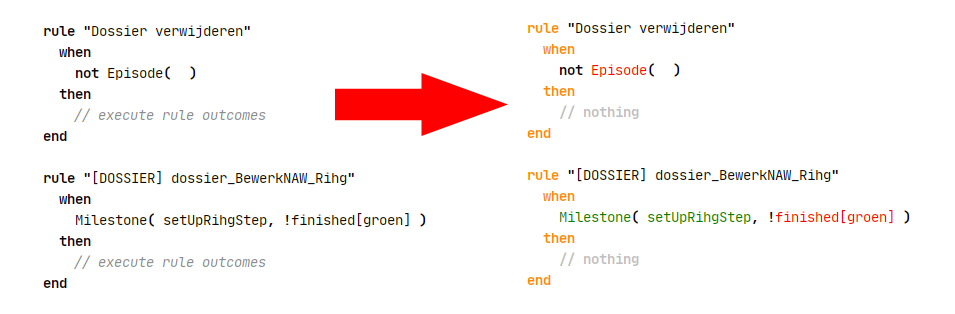
\includegraphics[width=0.99\textwidth]{Sections/images/coloredTextProjection.png}}
    \caption{Context aware color scheme}
    \label{fig:colorscheme}
\end{figure}

Facts that are contained by NotConditions and FactProperties that are part of a NotPredicate are highlighted in Red.
ExistConditions and IsPredicates have their content colored green.
We did not test whether this improved understanding.

\subsubsection{Summary projection}
Our next projection allows developers to have a quick overview of rules and complexity of those rules.
Figure \ref{fig:summaryProjection} shows that the developers are able to get an overview of both the number of rules and the number of facts in each of the rules.

\begin{figure}[h]
    \centering
    \fbox{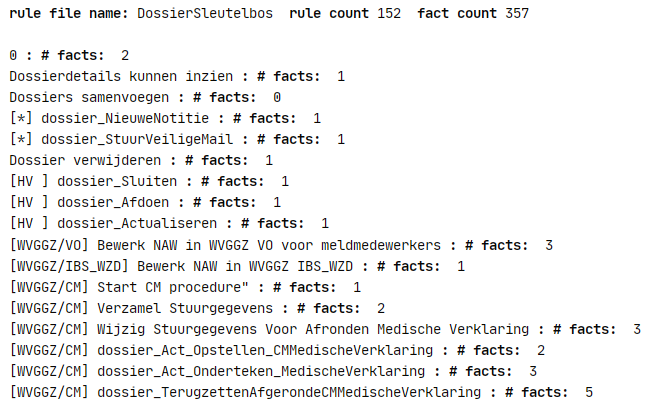
\includegraphics[width=0.75\textwidth]{Sections/images/summaryProjection.png}}
    \caption{Summary Projection}
    \label{fig:summaryProjection}
\end{figure}

The building of this rule only required adjusting two editors.
The rule count and fact count were added to the File editor using Read Only Model Access, to just count the descendants of the file that are rules and facts.
The rule editor was adjusted to only show the title of the rule and, again using the model access, the count of the descendants of the rule that were facts.

Whilst, this may look like a report, that any language workbench could create, the file name and all of the names of the rules are, in fact, still editable in this projection.

\subsubsection{Filtering}
The nature of business rules lends them to some projectional options that would not make sense with other programming styles.
because of the small, independent nature of the rules filtering in particular lends itself to the business rules style.
When looking at how to understand large files, we sought other domains than programming that handle large volumes of items.
The domain of data has a long history of handling large volumes.
Amongst their two most used tools for exploration are Sorting and Filtering.
On top of the semantic meaning of the ordering of the rules, we also did not imagine a good use case for sorting rules.
Thus de decided to implement a filtering projection.

Whilst filtering has been used in other places in the coding pipeline, such as in deciding on what code completion to present\cite{hou2010towards}, and version control visualization\cite{yoon2013visualization}, we were unable to find any research on applying filtering directly to code files.
Thus, we think what we present here is an original implementation.

When thinking about how business rules are related, one of the first things we look at is rules that examine the same facts or fact properties.
Thus these seemed the most obvious items to filter on.
We created a projection where if the developer filtered by a Fact or a Fact Property, then the projection would only filter out all rules that did not contain the item.
On top of this once the rules were filtered it would only show Facts and Fact properties that were used by those rules.

\begin{figure}[h]
    \centering
    \fbox{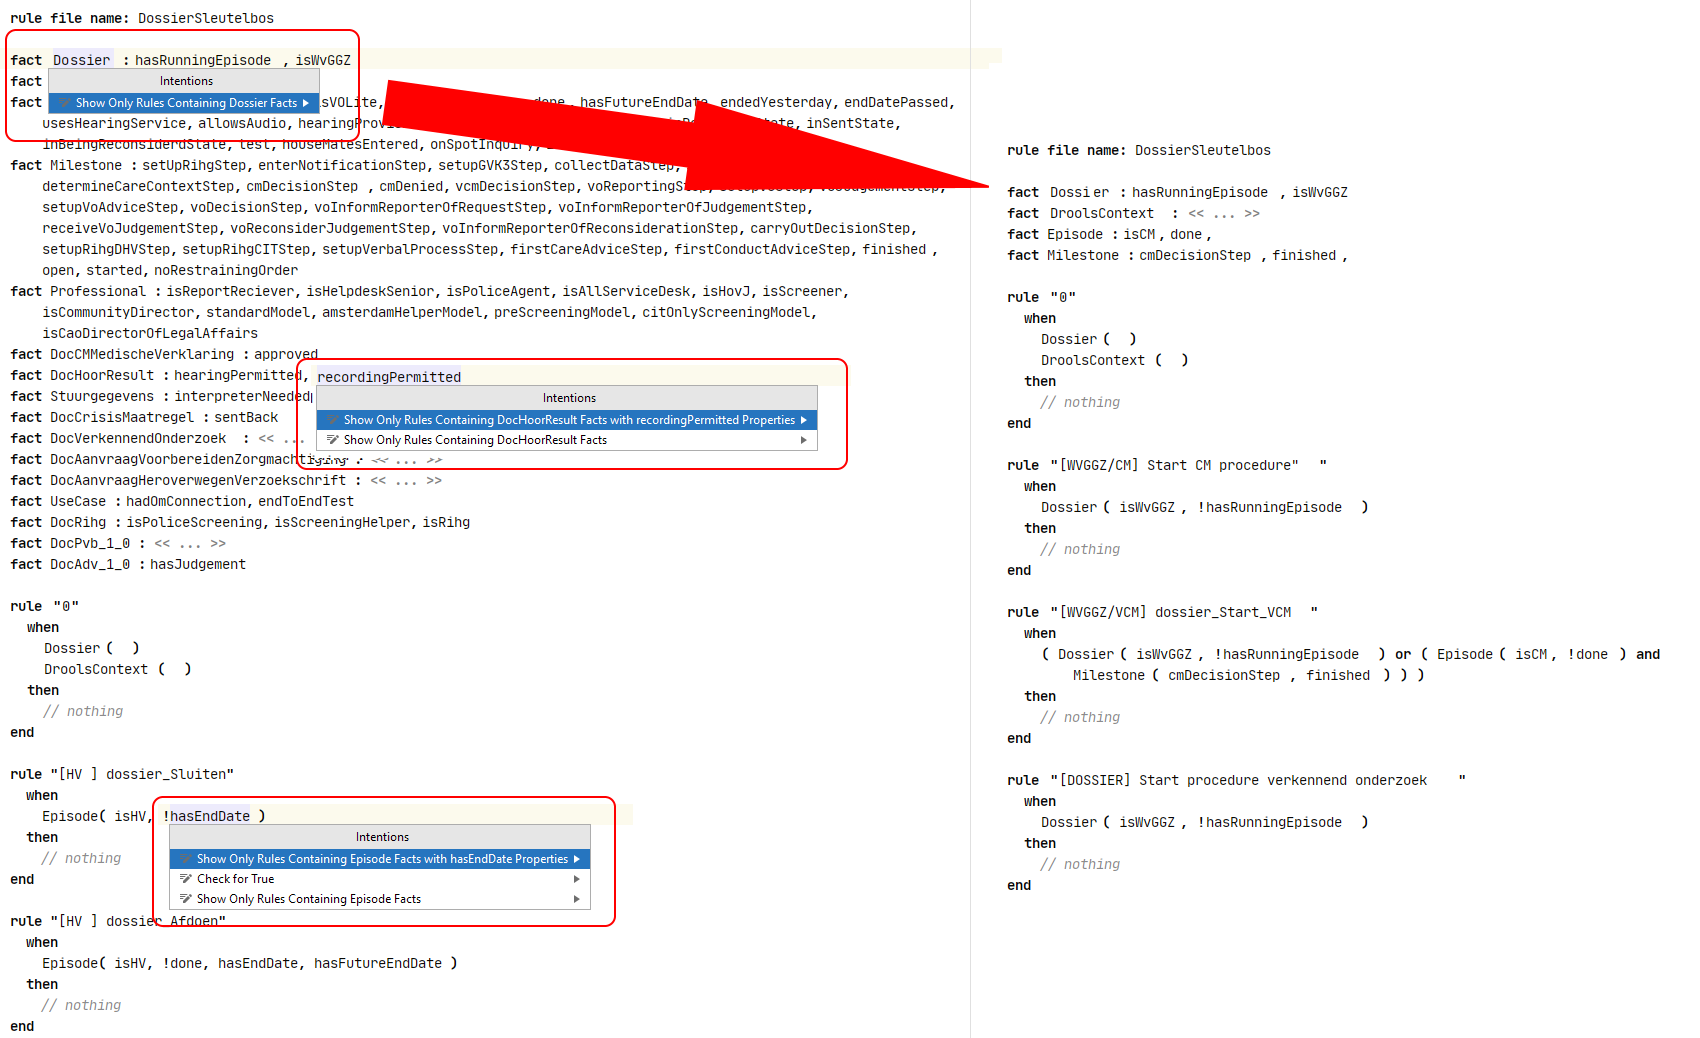
\includegraphics[width=0.99\textwidth]{Sections/images/filteringProjection.png}}
    \caption{Filtering Projection}
    \label{fig:filteringProjection}
\end{figure}

In our implementation, shown in figure \ref{fig:filteringProjection}, we show three places where we use intentions to filter the code.
The first is an intention on a Fact.
The outcome of choosing this filter is shown on the righthand side of figure \ref{fig:filteringProjection}.
The second intention is on a FactProperty.
As the FactProperty is a child of a Fact and we enabled that children could also show intentions, we also see an intention to filter on the parent Fact type.
The third highlighted intention is on a FactProperty Reference.
It also shows an intention for a Fact Reference in the FactSelector that holds the FactProperty reference as a child.

One of our guidelines for ourselves was, as much as possible, to build our projections as separate languages, non-invasively extending RSR.
Our first approach at the filtering, we failed on this count, by adding properties to Fact and FactProperty Concepts, to determine whether they were visible.

Our next approach created subclasses of Fact, FactProperty and File.
This however requires running a macro on the code file to migrate Facts, FactProperties and Files, to FilteredFacts, FilteredFactProperties, and FilteredFiles.
This means that the file could only be used by other languages that extend the filtered language.

Our Final approach was to add a Filter Concept and have that reference the filtered nodes, and have the editors make the visibility calculations based on this singleton node.
Whilst more complex, this removed the need for invasive changes and allowed other languages to combine with the filtering language.

Whilst this filtering is a handy projection, it does break Dijkstra's rule ``the purpose of abstraction is not to be vague but to create a new semantic level in which one can be absolutely precise.''\cite{dijkstra1972humble}.
The Summary projection could have been extended, so that the inspector contained all of the details of a selected rule.
This projection has no way of containing the whole code whilst a filter is applied.
However, so long as there is a clear indication that a filter is applied, then I do not see this as more of a problem than code collapsing found in most modern day editors.

\subsubsection{Table}
Thus far our projections have been textual ones that can be imagined with other language workbenches.
Creating a table will be our first non-parseable projection.
Our choice for this projection is based on the of Miller's\cite{miller1956magical} observations about the number of items people can retain in their memory.
Based on this observation then the counter-measure to this is to have fewer items off the screen and therefore in the developers memory.

\begin{figure}[h]
    \centering
    \fbox{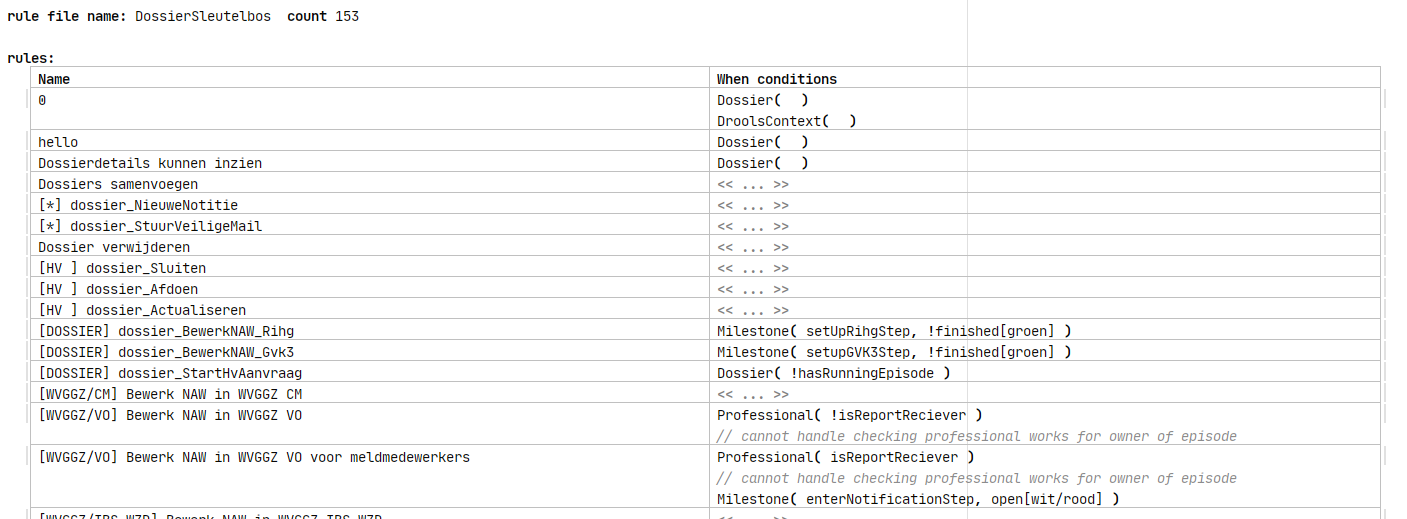
\includegraphics[width=0.99\textwidth]{Sections/images/tableProjection1.png}}
    \caption{Table Projection}
    \label{fig:tableProjection1}
\end{figure}

Figure \ref{fig:tableProjection1}, shows our rudimentary first table.
This simple table has only the Name property and the when children of the rules in the file.
This is implemented using the table extension, in the MPS-Extension Plugin, created by Sascha Lißon.

\subsubsection{Cross-Tab}
Our next tabular projection is a cross-tab inspired by a decision table.
The idea for this is that the previous table does not give any visual queues as to how rules are related.
With a cross-tab one can easily see which rules are using the same Facts.

\begin{figure}[h]
    \centering
    \fbox{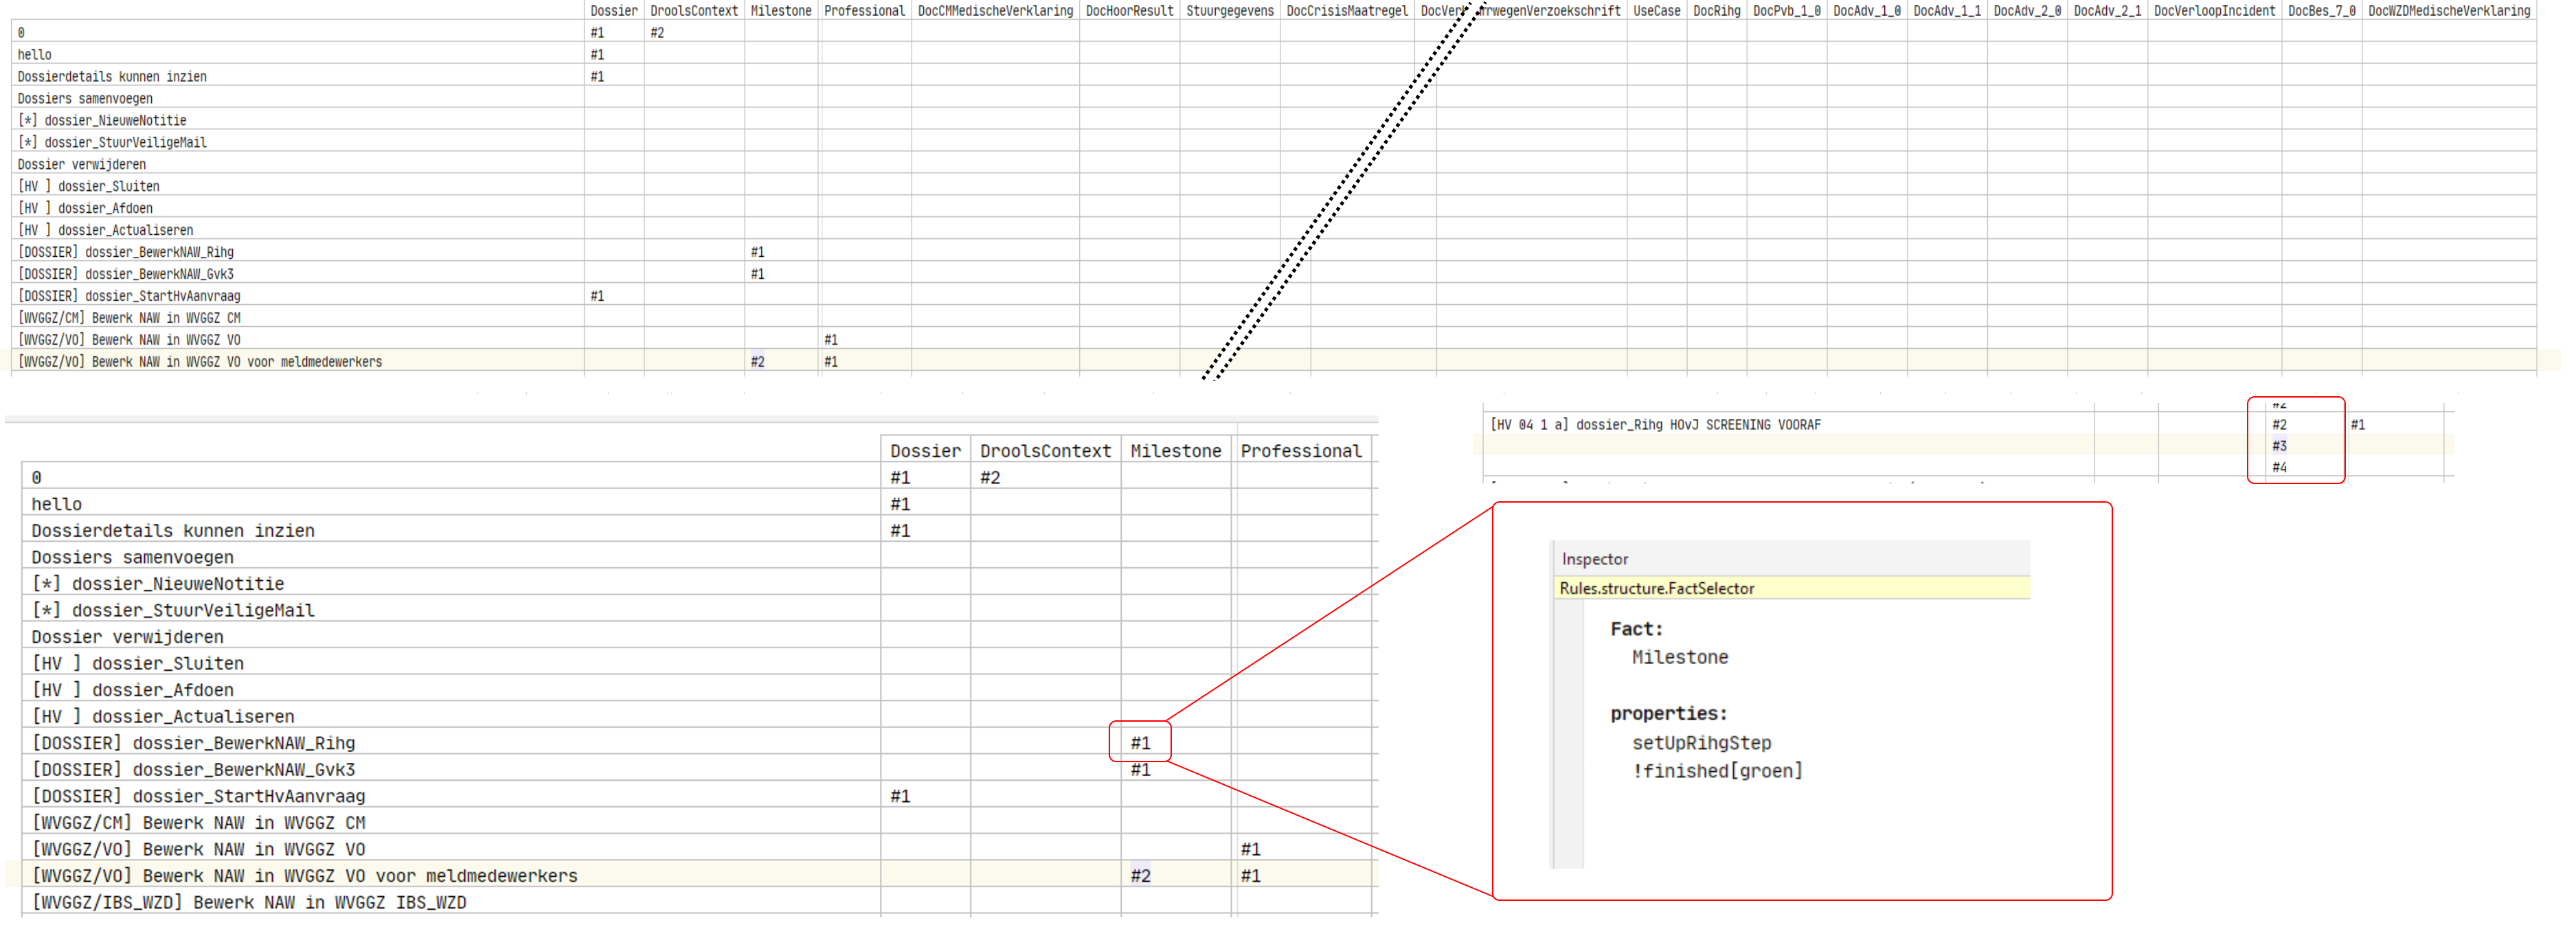
\includegraphics[width=0.99\textwidth]{Sections/images/crosstabProjection1.png}}
    \caption{Cross-Tab Projection}
    \label{fig:crosstabProjection1}
\end{figure}

Figure \ref{fig:crosstabProjection1} Shows our implementation of the cross tab.
At the top we can see an immediate problem with a cross-tab, and that is, if we have the whole file included the table will be very sparse.
Figure \ref{fig:crosstabProjection1} also has a close-up of a cell showing a rule using three FactSelectors that reference the same fact.
The other close-up shows that all the details of the selected fact are available in the inspector.

The sparse table would not be a problem if the columns are thin enough to keep the table in a single screen width.

Everything is editable in this table, including deleting the fact from the rule.
Most of the editing was provided by default by either MPS or the table plugin.
An extra editing feature we added to this table was the ability to delete a Fact from the file, and thus deleting all references to it from all the rules in the file, by deleting a Fact column column.
The code shown in figure \ref{fig:tableFactDeletion}, shows how we can walk the trees in each rule to delete unary conditions and convert the non-deleted side of binary conditions into unary conditions.

\begin{figure}[h]
    \centering
    \fbox{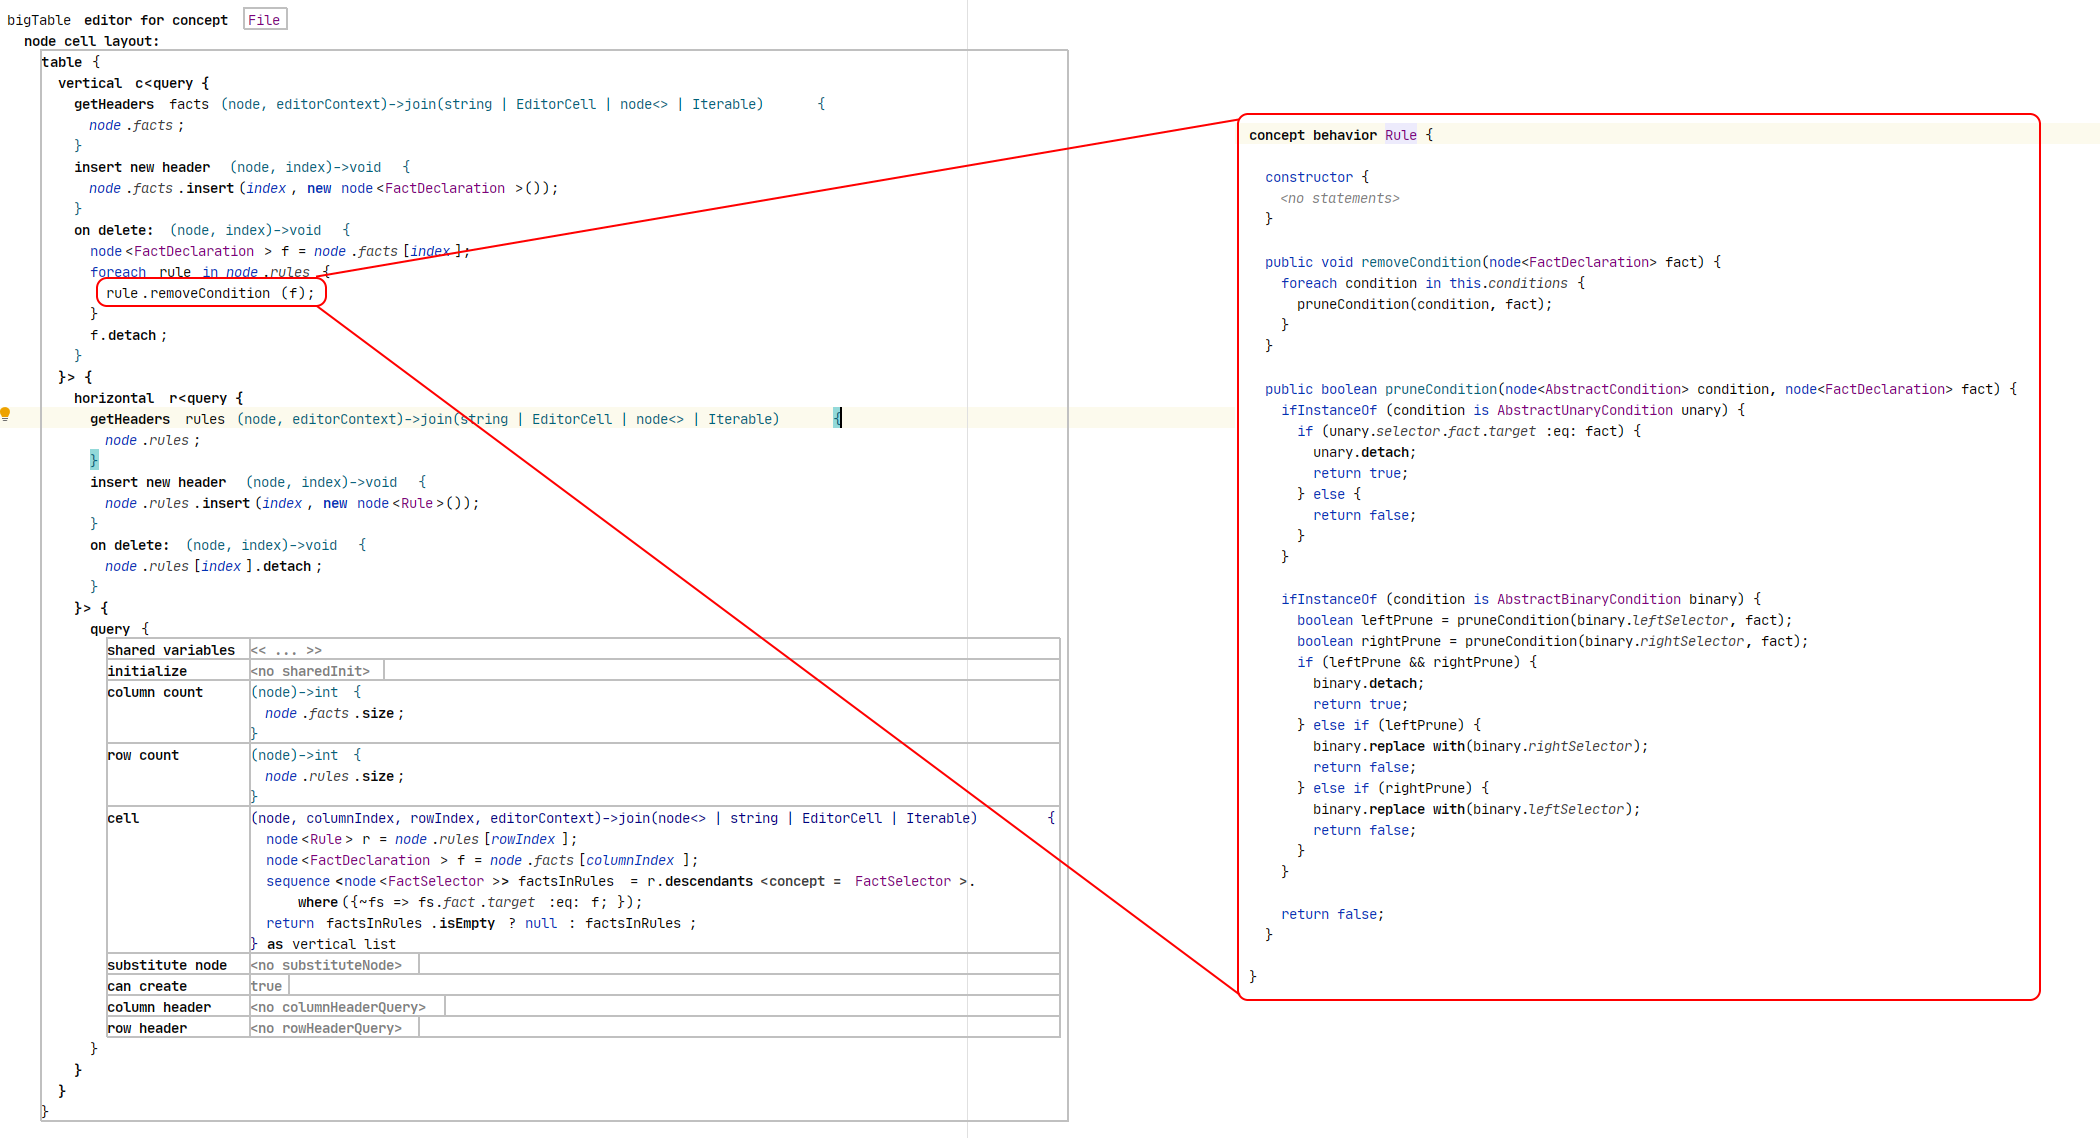
\includegraphics[width=0.99\textwidth]{Sections/images/tableDeleteCode.png}}
    \caption{Table fact deletion code}
    \label{fig:tableFactDeletion}
\end{figure}

Here ends our experiments in the RSR language.

\subsection{Drools-Lite}

Our next experiments were with projections with the Drools-Lite language.
As described in the section \ref{section:DroolsLite}, is an implementation that is much closer to the full Drools language.
These are the projections that we will present to experienced Drools developers for evaluation.

Of the learnings from the RSR language, one we felt needed to be fixed to aid understanding was the sparseness of the tables.
By implementing the principle of maximising cohesion, we discovered we could reduce the sparseness issue.
Thus, as a precursor to our projections, we extended Drools-Lite with a new language that contained one structural item, the Rule Collection.
The rule collection sits at the file level and holds a collection of rule statements.
The idea behind this is that rules that are related can be placed in the rule group so that it is easier to examine them together.
This language also had a default editor, and intentions to move rules in and out of groups.

\subsubsection{Decision Table}

As the Drools Language is analogous to a series of it-then-else statements, then perhaps it's best visual equivalent is the decision table.
It has long been shown that decision tables are a ``powerful aid in programming, documentation, and in effective man-to-man and man-to-machine communications''\cite{pooch1974translation}.

We designed our table, shown in figure \ref{fig:decisionTableProjection}, to include some of the lessons learned from the RSR CrossTab that was demonstrated in figure \ref{fig:crosstabProjection1}.
The RSR language taught us that sparseness in tables is exacerbated through wasting of visual real estate.
In the crosstab table, horizontal scrolling was necessary in part due to the column widths.
The columns were wide as the name of the Fact was displayed horizontally.

The Drools-Lite language allows for much longer selection criteria on Fact Properties, so we had to design the display with this in mind.
This screen real estate needed to be saved, as our decision table required a column to show the consequences of the selections, which in itself would be a wide column.
Our solution to this was to develop a vertically orientated header cell and use indentation to indicate if the cell is referring to just the Fact or a Fact and Fact Property combination.
The text for the header cells are generated based on the current


\begin{figure}[h]
    \centering
    \fbox{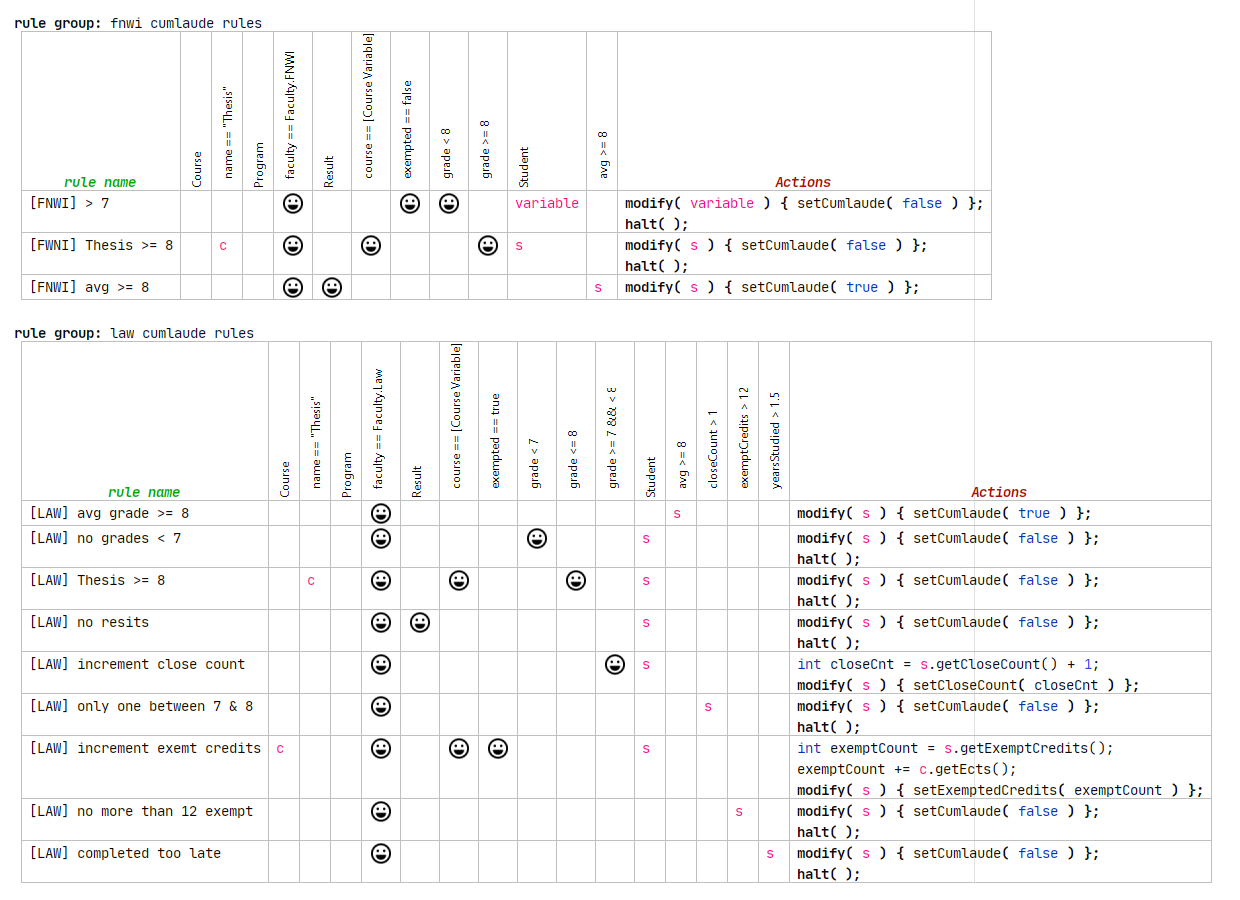
\includegraphics[width=0.99\textwidth]{Sections/images/decisionTableProjection.png}}
    \caption{Decision table projection}
    \label{fig:decisionTableProjection}
\end{figure}

Because this projection presents both the left and right hand side of the rules, we had to handle the Concept that spans both of these - the RuleVariable.
As the RuleVariable can be bound and used on the LHS as well as being used on the RHS, we had to find a way of representing this.
This was achieved by allowing a variable name to be used in the cell that represented the Fact or FactProperty it represented.
This lead to a happy visual design choice.
With variables now being represented in the cells, we could no longer represent the cell being selected with an 'X', as this could lead to confusion as to the meaning.
Projectional editing does not require meaning to be communicated with ASCII text.
Thus we decided to represent selection with an image, and personal preference and a misspent youth lead us to the smiley face as that indicator.

The rule names and actions are editable through the default functionality of the MPS extension.
Adding a selection criteria to a rule occurs through an intention attached to the associated cell, as is also the case for binding a variable.

The major drawback of this design is that editing a rule with an as yet non-existent selection criteria became very clunky.
If the rule we wished to edit already existed in the table we had to use an intention to extract it from the group change the criteria and place it back in.
At this point the table would automatically adjust the column headings.

This design was examined by experts in the questionnaire.

\subsubsection{SpreadSheet}

The domain specific language for the finance world is the spreadsheet.
One study estimated that 90\% of computers had a spreadsheet on them\cite{bradley2009using}.
It has been suggested that Dan Bricklin's VisiCalc is the reason for the success of PC's in The office.
VisiCalc was succeeded by Lotus 1-2-3, which in turn was succeeded by Microsoft Excel as the dominant Spreadsheet program in the workplace.

This level of familiarity to a paradigm lead us to try to design a projection that had the same look and feel of an Excel spreadsheet.
This design can be seen in figure \ref{fig:SpreadsheetProjection}.
To this end we created a design where the selection criteria could be directly edited in the cell, as highlighted in the figure.

\begin{figure}[h]
    \centering
    \fbox{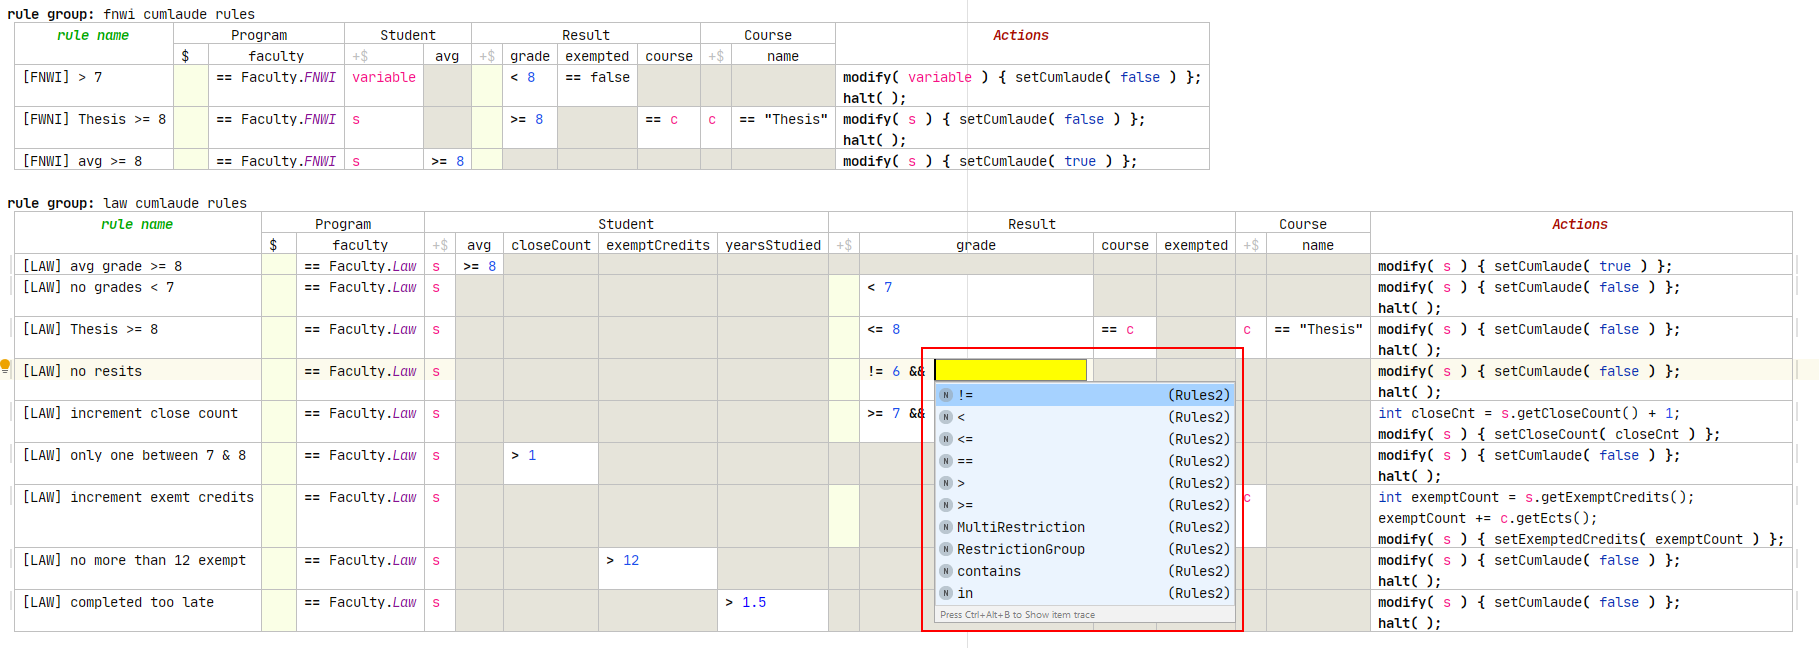
\includegraphics[width=0.99\textwidth]{Sections/images/SpreadsheetProjection.png}}
    \caption{Spreadsheet projection}
    \label{fig:SpreadsheetProjection}
\end{figure}

In this design each row is a rule, each column is for a variable or a property of a fact.
If a property is selected then the selection criteria is in the appropriate cell.
Unselected cells are indicated by a grey/beige color.
The RHS of the rule appears in the Actions column.
To add as yet unused facts or fact properties, or remove existing ones, can be achieved with intentions, as shown in figure \ref{fig:SpreadsheetIntentions}.

This Design also allowed us to have more than one selector for the same FactProperty, this being important for our host organizations code.
This is demonstrated in the figure \ref{fig:TwoProperties}.

\begin{figure}
    \centering
    \begin{minipage}{0.35\textwidth}
        \centering
        \fbox{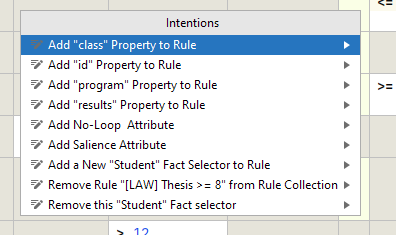
\includegraphics[width=0.95\textwidth]{Sections/images/spreadsheetIntentions.png}}
        \caption{Intention}
        \label{fig:SpreadsheetIntentions}
    \end{minipage}\hfill
    \begin{minipage}{0.65\textwidth}
        \centering
        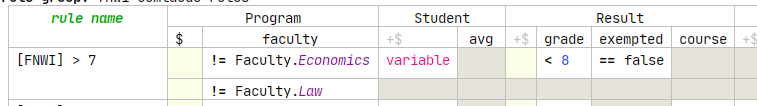
\includegraphics[width=0.95\textwidth]{Sections/images/spreadsheetTwoProperties.png} 
        \caption{Two of same Property}
        \label{fig:TwoProperties}
    \end{minipage}
\end{figure}

This design was examined by experts in the questionnaire.

Here ends our experiments in the Drools-lite language.

\subsection{Wireframe}

After brainstorming several ideas to present as wireframes to experts as possible projectional aids to understanding we chose two.
We discuss them briefly in this section.

\subsubsection{Truth Table}
We decided to produce this example as we had had experience of building truth tables to confirm the validity of Drools rules in our work, thus we had an n of 1 whom we knew would find this projection useful.

The truth table seemed apt for the LHS of the Drools rule as in essence it is a boolean function.
Wittgenstein popularized the truth table in the Tractatus Logico-Philosophicus\cite{wittgenstein2013tractatus}.
It is so widely used in mathematics and computer science, that we do not feel the necessity to explain its use further.
Because of the combinatorial explosive nature of truth tables, with 2\textsuperscript{n} possible combinations, thus we would limit display to a max of 6 variabiables and only show the paths that lead to the RHS being executed.

\begin{figure}[h]
    \centering
    \fbox{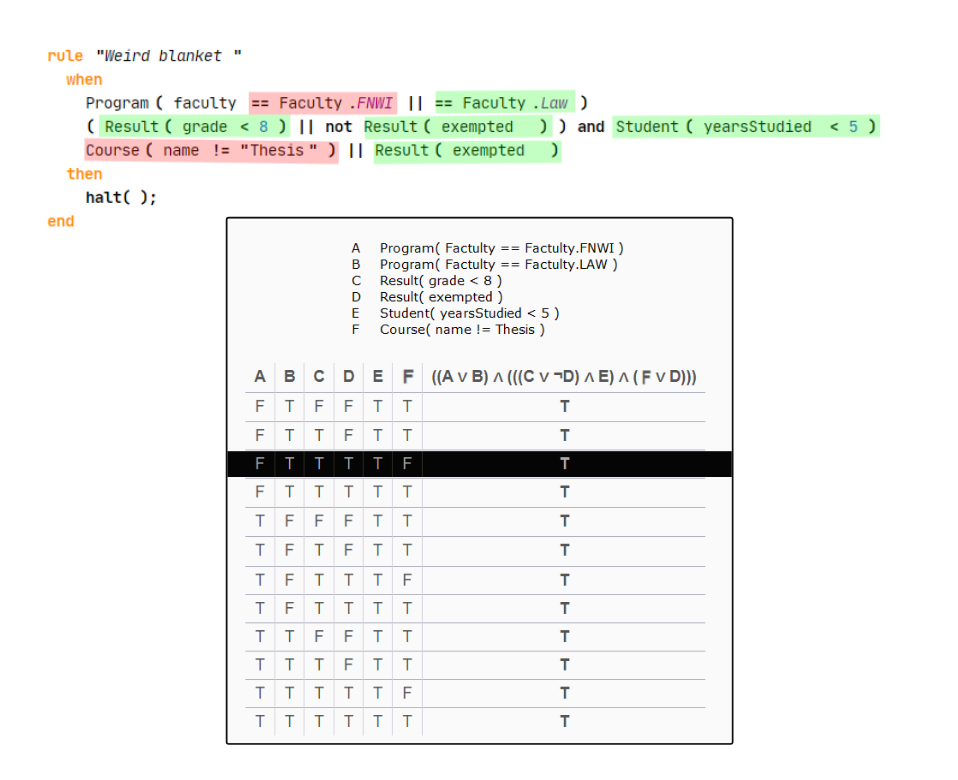
\includegraphics[width=0.80\textwidth]{Sections/images/truthtable.png}}
    \caption{Truth Table Projection}
    \label{fig:TruthTableProjection}
\end{figure}


Figure \ref{fig:TruthTableProjection} shows how we designed this to look.
The user experience would be that the rule is selected and the developer presses the up and down arrow keys to step through the different true (highlighted in green) and false (highlighted in red) fact selections that result in a true outcome.

We presented this design to our experts through the questionnaire to be validated.

\subsubsection{Circuit Diagram}
Our last projection design wanted to present a part of projectional editing that we had heretofore only mad minimal use of.
That is the use of Graphics which can be manipulated to change the AST.

We chose a logic circuit. The logic circuit represents a boolean operations as NOT, OR, XOR and AND Gates with their inputs and outputs being inputs to other gates.
In our design, shown in figure \ref{fig:CircuitDiagramProjection} the input wires to the gates are the Facts or FactProperties referenced in the LHS.

\begin{figure}[h]
    \centering
    \fbox{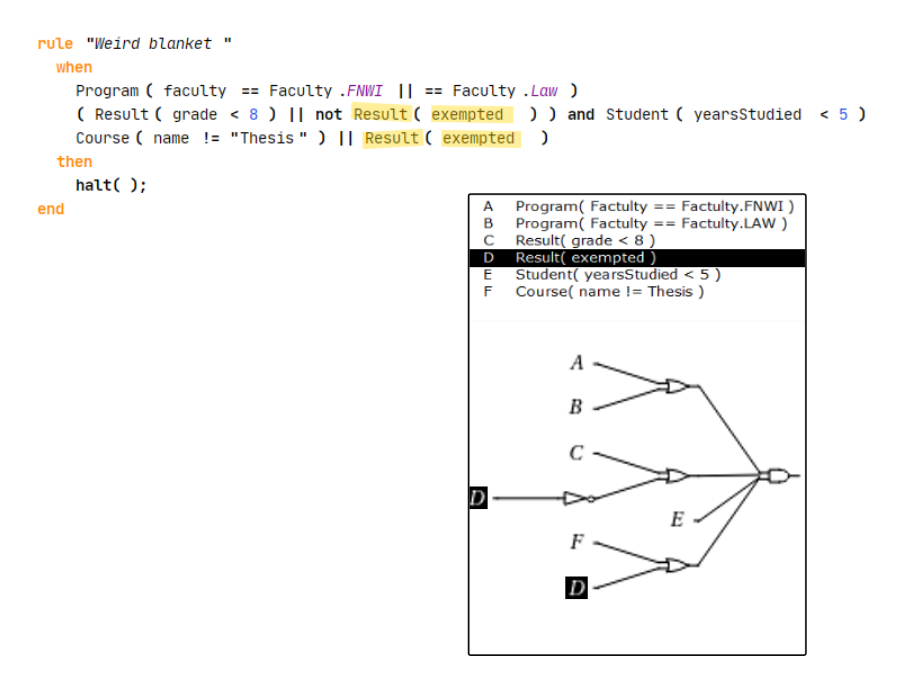
\includegraphics[width=0.80\textwidth]{Sections/images/CircuitDiagram.png}}
    \caption{Circuit Diagram Projection}
    \label{fig:CircuitDiagramProjection}
\end{figure}

The user experience is that once the rule is selected, the developer, by pressing the up and down arrow keys, can step through the different fact selections (highlighted in yellow) and shown in the circuit diagram, thus showing how the facts relate to each other.

This design is also presented in the questionnaire for validation.

